


\tikzset{every picture/.style={line width=0.75pt}} %set default line width to 0.75pt        

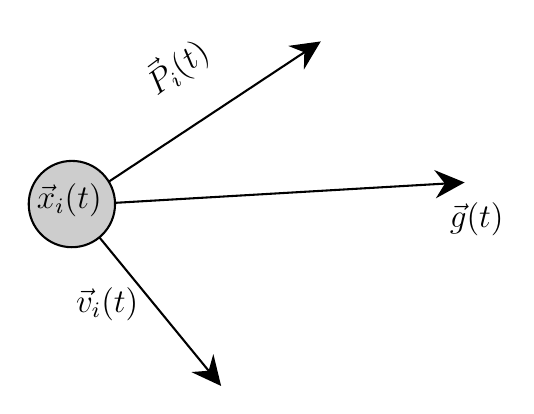
\begin{tikzpicture}[x=0.75pt,y=0.75pt,yscale=-1,xscale=1]
%uncomment if require: \path (0,300); %set diagram left start at 0, and has height of 300

%Straight Lines [id:da7251476173740483] 
\draw    (212,118) -- (397.61,107.17) ;
\draw [shift={(400.61,107)}, rotate = 176.66] [fill={rgb, 255:red, 0; green, 0; blue, 0 }  ][line width=0.08]  [draw opacity=0] (14.29,-6.86) -- (0,0) -- (14.29,6.86) -- (9.49,0) -- cycle    ;
%Straight Lines [id:da18169270686596173] 
\draw    (212,118) -- (328.81,40.71) ;
\draw [shift={(331.31,39.05)}, rotate = 146.51] [fill={rgb, 255:red, 0; green, 0; blue, 0 }  ][line width=0.08]  [draw opacity=0] (14.29,-6.86) -- (0,0) -- (14.29,6.86) -- (9.49,0) -- cycle    ;
%Straight Lines [id:da054979634098808905] 
\draw    (212,118) -- (281.41,202.73) ;
\draw [shift={(283.31,205.05)}, rotate = 230.68] [fill={rgb, 255:red, 0; green, 0; blue, 0 }  ][line width=0.08]  [draw opacity=0] (14.29,-6.86) -- (0,0) -- (14.29,6.86) -- (9.49,0) -- cycle    ;
%Shape: Circle [id:dp6795888605590055] 
\draw  [fill={rgb, 255:red, 205; green, 205; blue, 205 }  ,fill opacity=1 ] (190.61,117.4) .. controls (190.61,105.92) and (199.92,96.61) .. (211.4,96.61) .. controls (222.89,96.61) and (232.2,105.92) .. (232.2,117.4) .. controls (232.2,128.89) and (222.89,138.2) .. (211.4,138.2) .. controls (199.92,138.2) and (190.61,128.89) .. (190.61,117.4) -- cycle ;


% Text Node
\draw (392,115) node [anchor=north west][inner sep=0.75pt]  [font=\large]  {$\vec{g}( t)$};
% Text Node
\draw (193,106) node [anchor=north west][inner sep=0.75pt]  [font=\large]  {$\vec{x}_{i}( t)$};
% Text Node
\draw (241,52.96) node [anchor=north west][inner sep=0.75pt]  [font=\large,rotate=-323.22]  {$\vec{P_{i}}( t)$};
% Text Node
\draw (212,156) node [anchor=north west][inner sep=0.75pt]  [font=\large]  {$\vec{v}_{i}( t)$};


\end{tikzpicture}